\chapter{Background}
\label{cha:background}
This chapter presents the background of the thesis. On the one hand, we describe the RoboCup and LLSF in section~\ref{sec:robocup} and the Robotino in section~\ref{sec:robotino}. On the other hand, we present the most important software for this thesis. In section~\ref{sec:robot_software_frameworks} we present the two robot software frameworks ROS and Fawkes. Section~\ref{sec:gazebo} describes the robot simulator Gazebo, followed by additional software in section~\ref{sec:additional_software} which includes the data exchange format Protocol Buffers, the CLIPS Rules Engine and the document database MongoDB.

\section{RoboCup}
\label{sec:robocup}
The \textit{RoboCup}\footnote{\url{http://www.robocup.org}} is an international robotics competition founded in 1997~\cite{Robocup}. It provides standard problems as a platform for artificial intelligence and robotics research. Research teams from all over the world compete in different leagues to benchmark their robotic system. The RoboCup provides a research test-bed, in which participating teams implement new approaches and make them robust against the challenges of the real world complexity. Furthermore, the competition leads to comparison and evaluation of different approaches. Every year, the competition takes place at the RoboCup world championship, which is hosted by changing nations. There are also offshoots, such as the RoboCup GermanOpen in Magdeburg.\\
Initially, RoboCup started as a robot soccer world cup. The goal ``By mid-21st century, a team of fully autonomous humanoid robot soccer players shall win the soccer game, comply with the official rule of the FIFA, against the winner of the most recent World Cup.''~\cite{robocup_goal} shows how far the RoboCup is wants to push the development of artificial intelligence and robotics. Since then, RoboCup has grown and now features a variety of different leagues in different domains. In the following we give an overview of the RoboCup leagues in 2013:\\
\textbf{Soccer Leagues:} The majority of the RoboCup leagues are soccer leagues with different robot sizes and platforms. There is a \textit{Standard Platform League (SPL)} where the teams have to use about 60 cm high humanoid NAO robots without any hardware modifications. This enables the teams to focus on vision, behavior and motion tasks. There is also a league for other humanoid robots. This league is divided into three sub-leagues with kid, teen and adult size robots. The \textit{Middle Size League (MSL)} features up to five robots per team on a 18 m x 12 m field with each robot having a footprint smaller than 52cm x 52cm. In the \textit{Small Size League (SSL)}, there are six robots, each with a diameter up to 18 cm, per team.\\
\textbf{Soccer Simulation Leagues:} There are also two soccer simulation leagues which focus on artificial intelligence and team strategy instead of developing robot hardware. There are a 2D simulation league and a 3D simulation league. In the 3D simulation league, teams consisting of eleven virtual NAO robots compete against each other in a realistic soccer environment. In chapter~\ref{cha:related_work}, we show both simulations in detail.\\
\textbf{RoboCup@Home:} The RoboCup@Home league is a competition about service robots. The robots have to assist humans in a domestic environment. There are a variety of tasks, such as following a human, serving drinks and handling emergency situations. Especially important in this league are the technical and open challenge. Here, the teams can present their own ideas and how the robot implements them.\\
\textbf{Rescue League:} The rescue league is a test-bed for urban search and rescue robots. The robots have to find victims in a setup course that simulates an urban area after an earthquake. The league has high demands on robot hardware and is divided into several fields, such as autonomous robots and remote-controlled robots. \\
\textbf{Rescue Simulation Leagues:} There are also two rescue simulation leagues called \textit{Agent Competition} and \textit{Virtual Robot Competition}. In the Agent Competition many heterogeneous agents have to fight a large disaster in a city. The Virtual Robot Competition is about finding victims with a group of robots in a smaller area. We show both in chapter~\ref{cha:related_work} in more detail.\\
\textbf{RoboCup@Work:} The RoboCup@Work league targets working tasks with the YouBot. The YouBot is a mobile robot equipped with a five degree of freedom arm. The goal is to perform work-related tasks, such as identifying and handling different objects, placing them in bins and transportation.\\
\textbf{Logistic League:} We describe this league in detail in the following subsection.\\

\subsection{Logistic League sponsored by Festo}

\label{sec:llsf}
The Logistic League Sponsored by Festo (LLSF) is a competition within RoboCup. LLSF aims to foster scientific work on autonomous solutions for logistics and to provide a test-bed for existing approaches~\cite{LLSFTestbed}. The participants have to find new approaches and improve already existing ones to optimize material and information flow in logistics.
LLSF takes place  in a simplified production hall~\cite{LLSFRules}.
\begin{figure}
\begin{minipage}[b]{0.5\linewidth}
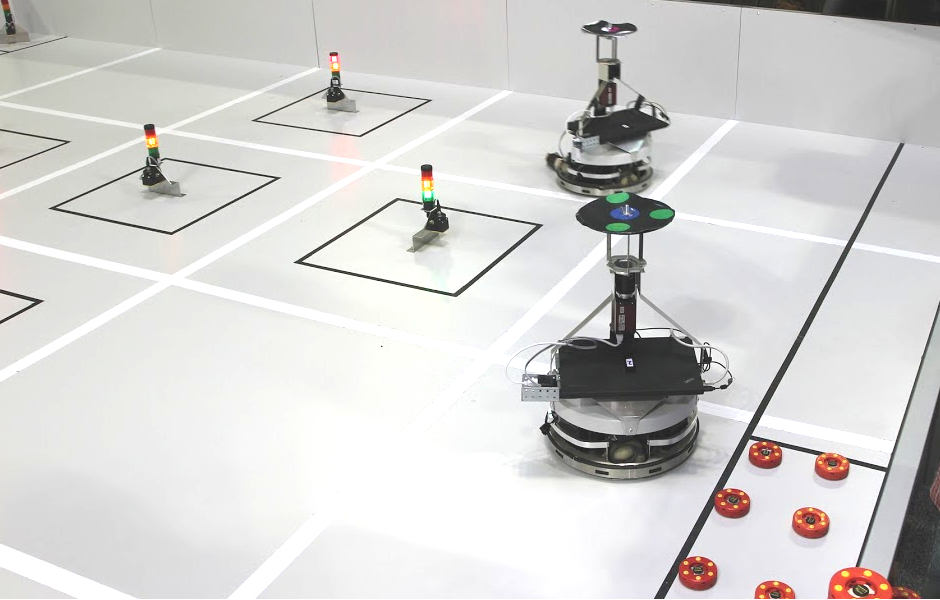
\includegraphics[scale=0.23]{pics/llsf}
\caption{Part of the LLSF field}
\label{fig:llsf_field}
\end{minipage}
\quad
\begin{minipage}[b]{0.5\linewidth}
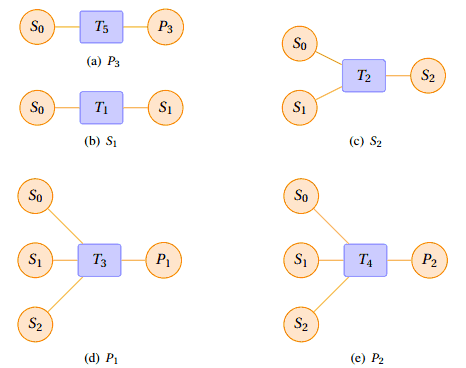
\includegraphics[scale=0.45]{pics/production_chain}
\caption{LLSF Production Chain~\cite{LLSFRules}}
\label{fig:llsf_chain}
\end{minipage}
\end{figure}
Figure~\ref{fig:llsf_field} shows a part of the 5.6m x 5.6m hall with two Carologistics robots, three machines and some material-pucks. The main task of LLSF is to produce and deliver ordered products as efficiently as possible by feeding machines with resources and semi-finished products. The participants can use up to three Robotino robots by Festo~\cite{{Robotino}}. We present the Robotino in the next
section in detail. Orange pucks represent resources and products. They are equipped with an RFID-chip\footnote{Radio-frequency identification allows the wireless identification of objects with small chips.}
which is needed to store the different product states of the pucks. The machines are represented by the RFID-readers with signal-lights on top. The signal-lights indicate the current status of a machine, such as ``ready'', ``producing'' and ``out-of-order''. The machines need resources and semi-finished products as input and turn the last input puck into a further processed puck. All other input pucks are turned
into consumed pucks which can be recycled to produce new resource pucks. There are different types of machines. The type defines the needed input and the produced output of a machine. Figure~\ref{fig:llsf_chain} shows the production chain. There are the raw-material pucks $S_0$, intermediate product pucks $S_1$ and $S_2$ and product pucks $P_1$, $P_2$ and $P_3$. The machine types are labeled with
$T_1$ to $T_5$. Beside these regular machines, there are also recycling machines, which turn consumed pucks into raw-material pucks, and delivery machines which are used for delivering finished product pucks. Teams are awarded with points for delivering finished products, producing complex pucks and recycling. The game is divided into two phases. In the first phase, the \textit{exploration phase}, the robots have three minutes to explore the production area to identify which machine is of which type. Teams also receive points for each correctly reported machine-type. The second phase is the actual \textit{production phase} and lasts 15 minutes. The league also features an automated referee box (Refbox) which realizes the logic behind the LLSF environment. It controls machines and communicates with participating robots during the game. The Refbox gives orders which products are to be produced, informs the robots about the game state and rewards points for achieved goals.


\section{Robotino}
\label{sec:robotino}
\begin{figure}
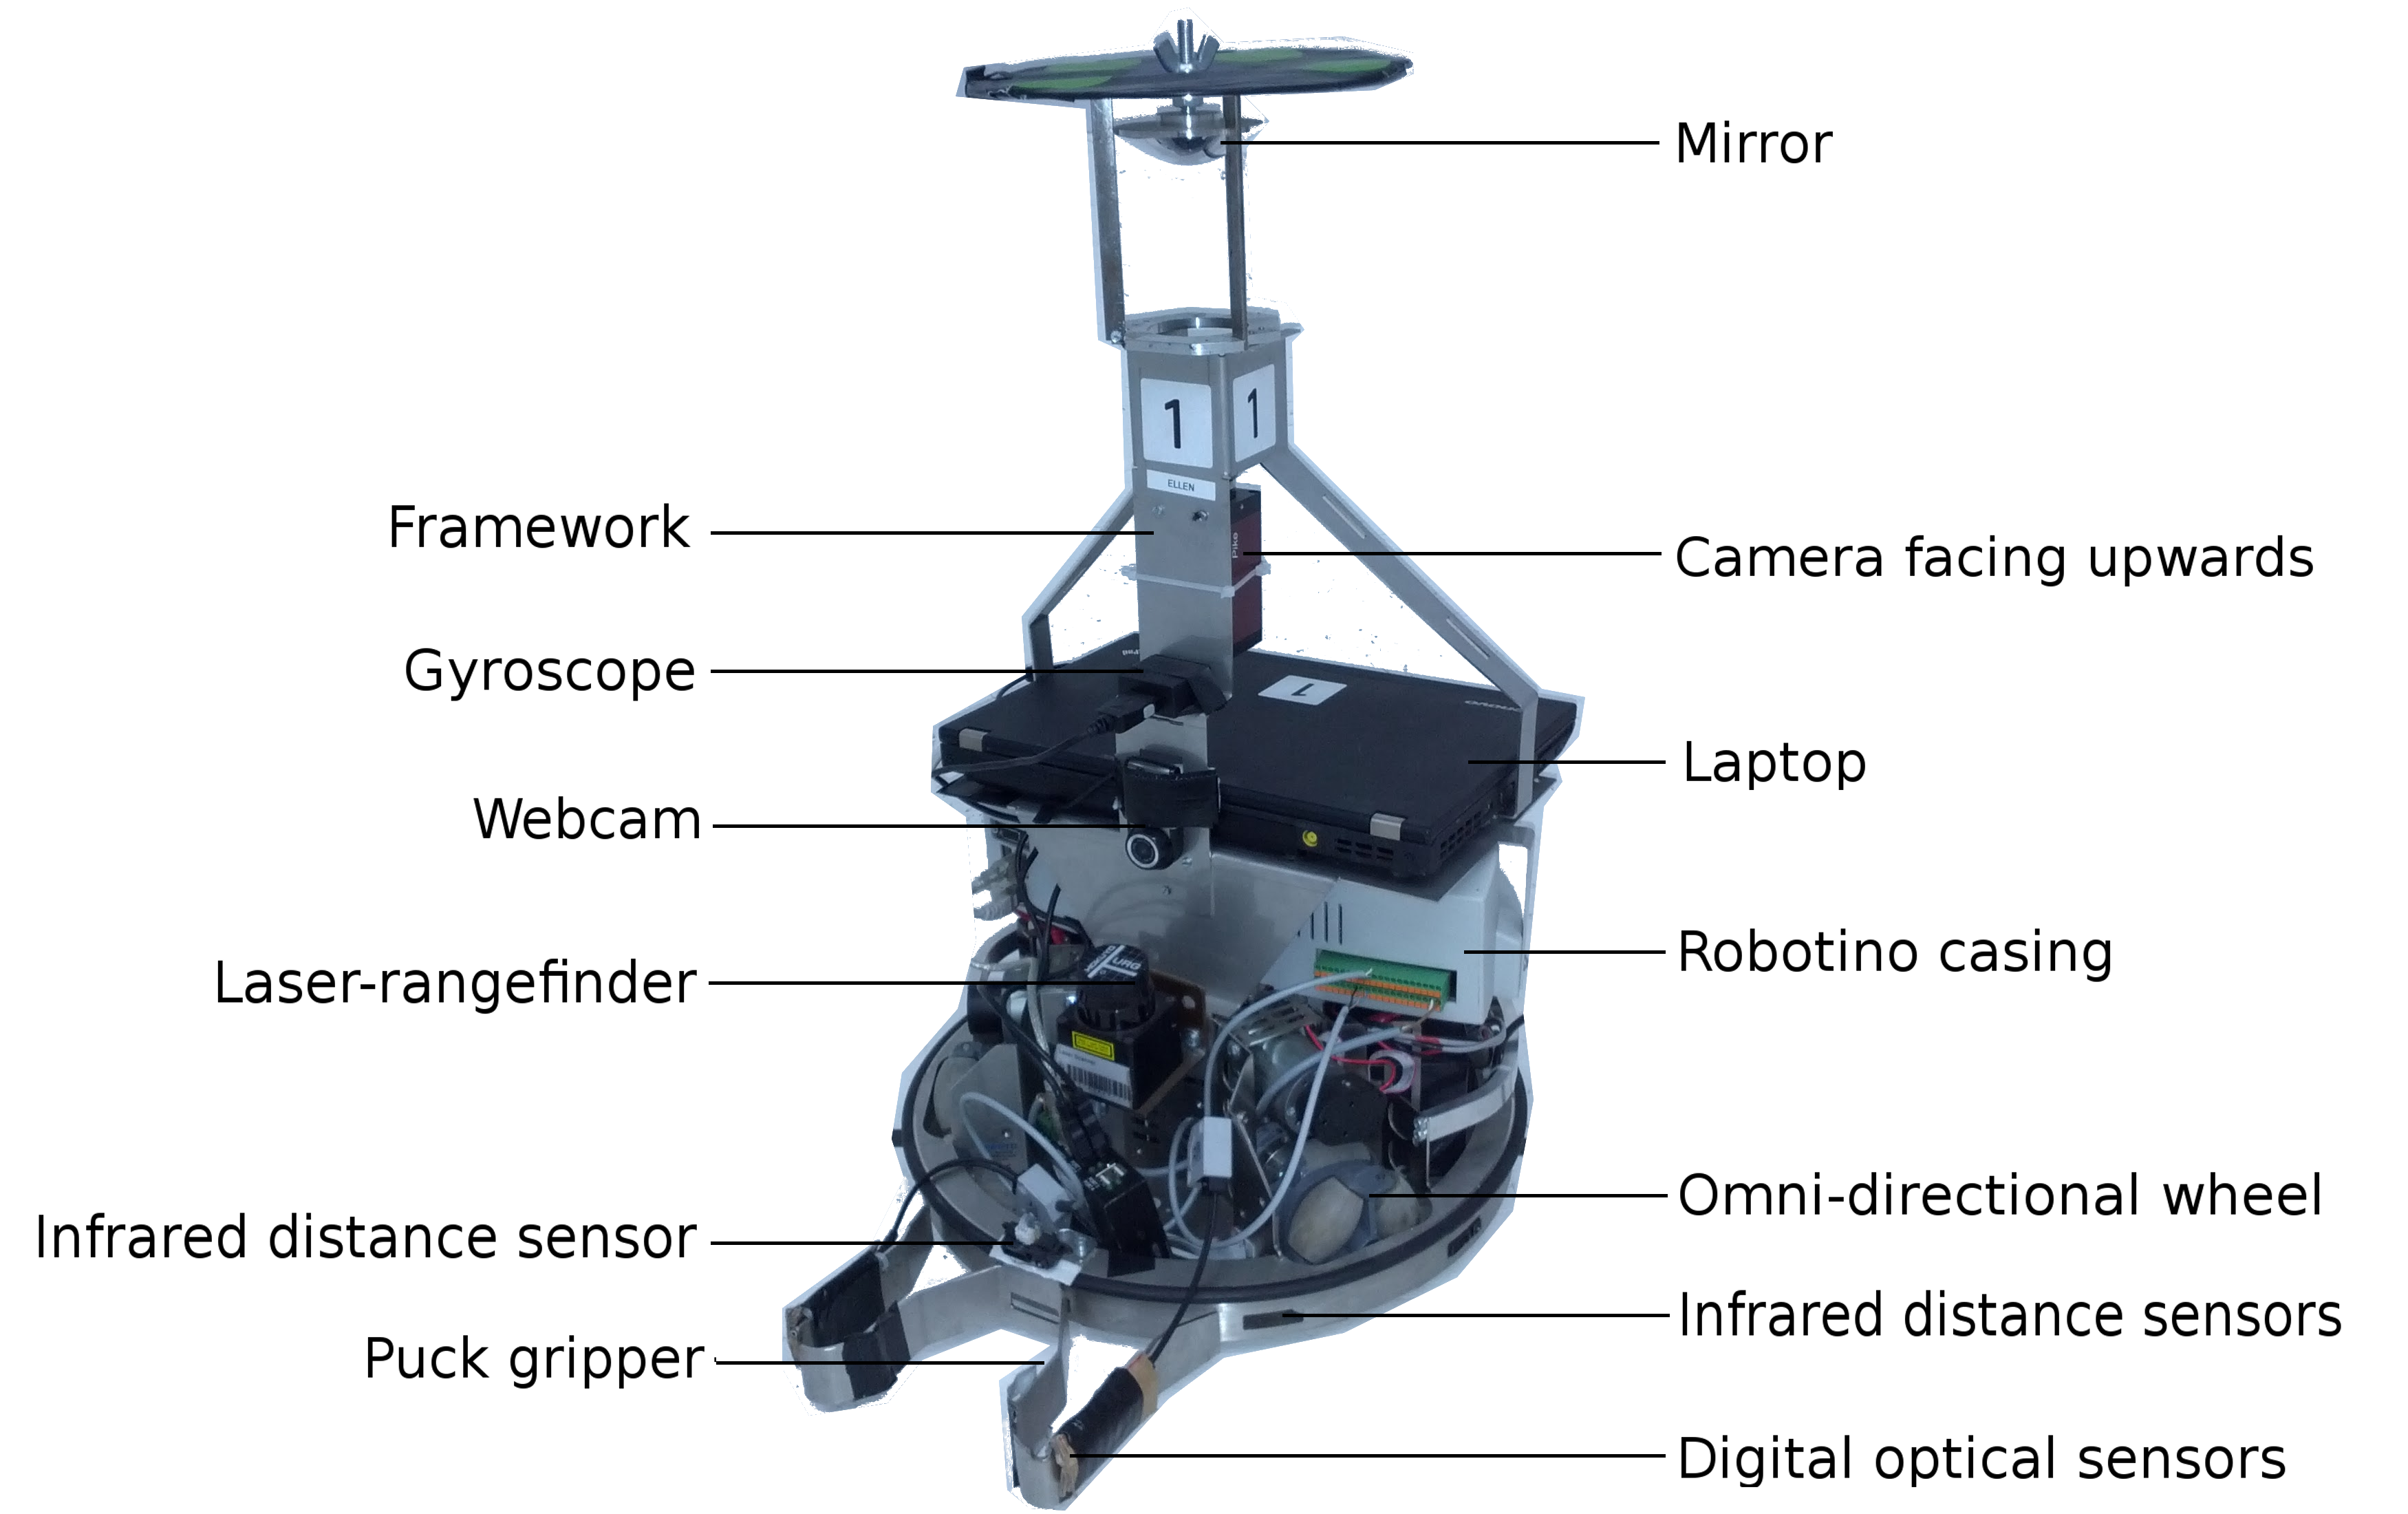
\includegraphics[scale=0.11]{pics/carologistics_robotino}
\caption{A Robotino extended by Carologistics}
\label{fig:caro_robotino}
\end{figure}
The \textit{Robotino}~\cite{Robotino} is a mobile robot developed by Festo Didactic\footnote{\url{http://www.festo-didactic.com}}. It is used for research and education. The shape of the Robotino is a cylinder with 37cm diameter and 21cm height. It has omni-directional wheels to be able to drive in any direction and turn at the same time. It is equipped with nine infrared distance measuring sensors ordered around the robot, a bumper to detect collisions and a webcam. A micro-controller and an embedded PC with 500 MHz and 256 MB RAM are used to control the robot~\cite{Incremental}. The PC runs with a Linux Operating System. The Robotino is designed to be extendable to be used in different applications. Therefore additional sensors and actuators can be attached. At the front of the Robotino, there is a loading bay with some space for extensions. Figure~\ref{fig:caro_robotino} shows a Robotino extended by Carologistics. In addition to the default sensors shipped with the Robotino, we added a laser-rangefinder for localization and obstacle detection, a gyroscope and a framework which holds an omni-directional camera. The omni-directional camera consists of a camera facing upwards and a hyperbolic mirror above. The camera can see the whole area around the Robotino through the mirror. We adapted the omni-vision camera from former MSL-robots and now use it to detect LLSF pucks. The framework also holds a laptop connected to the Robotino, because we need more computational power than the Robotino provides for localization and path planning. We also attached a simple puck holder to the front. This puck holder is equipped with an infrared distance sensor to recognize if there is a puck in the holder and a digital optical sensor on each side of the puck holder. These are used to align the robot in front of LLSF machines. To observe the signal-lights on the machines, we use a webcam.\\


\section{Robot Software Frameworks}
\label{sec:robot_software_frameworks}
A robot software framework is a design and implementation which acts as a middleware and provides functionality and tools for the implementation of a robot control software~\cite{tnthesis}. In the following, we present Fawkes and ROS, which are the two robot software frameworks used in this thesis.

\subsection{Robot Operating System}
The \textit{Robot Operating System (ROS)}\footnote{\url{http://www.ros.org}} is an Open Source framework designed to operate on many robot platforms and to provide a standardized integration framework~\cite{Ros}. It provides a collection of useful Open Source libraries and tools for the development process of robot-software. Currently, it is widely used and has a large community. Each component integrated in ROS runs an own process and is called \textit{node}. ROS features peer-to-peer communication between nodes. Nodes can register a publisher or subscriber to a specified \textit{topic}. If a publisher of a topic sends a message, every subscriber of same topic receives the message. We will describe the message protocol Google Protobuf used by ROS later. The communication is managed by a process called \texttt{roscore}. \texttt{roscore} acts as a topic registry server. All nodes have to connect to the server in order to operate.\\
We use ROS in LLSF for two reasons. First, we use ROS for motion planning. The ROS package \texttt{move\_base} provides a global path planning and local motion planning with collision avoidance. We provide the position and orientation of the robot, laser data for obstacle detection and motion goals by publishing messages to specified topics. With this data, \texttt{move\_base} computes a motor command. We subscribe to the motor command topic and execute received commands. Second, we use the \texttt{rviz} package for visualization. For example, we visualize incoming laser data, the localization of the robot and motion plans. Moreover, we use \texttt{rviz} to send localization hints to the robot.

\subsection{Fawkes}
\textit{Fawkes}\footnote{\url{http://www.fawkesrobotics.org}} is an Open Source robot software framework developed primarily at the Knowledge-based Systems Group\footnote{\url{http://www.kbsg.rwth-aachen.de}} (KBSG) at RWTH Aachen University~\cite{FawkesDesign}. It is designed to run on multiple platforms and domains. It is written for Unix systems and follows a component-based software design~\cite{component}. It provides an infrastructure to load and unload binary components (implemented as \textit{plugins}) at run-time. Fawkes features a \textit{blackboard} as communication structure between plugins. The blackboard lists structured entries called \textit{interfaces}. Plugins are composed of thread, which can read and write interfaces with a specified id. There can be many readers but only one writer for an interface. Furthermore, Fawkes organizes plugin activity in threads to make use of multi-core architectures. Because of this design, Fawkes is flexible and dynamic. The interchangeability of the plugins, which is caused by well defined interfaces, makes hardware abstraction and reuse easy. This is also an important advantage for the development of the simulation because the simulation can easily exchange lower-level robot control and sense plugins. Then, robot control plugins on higher levels can operate as on the real robot because the interface is the same. The features of Fawkes are provided as \textit{aspects}. These aspects are based on aspect-oriented programming~\cite{aspect_oriented} and give access to a particular feature. Threads that want to use a feature can inherit from the corresponding aspect. For example there are aspects for accessing the blackboard, logging and timing~\cite{tnthesis}. In this thesis, we give access to communication with the simulation by providing such an aspect. Two other important features for this thesis are the centralized clock and the configuration. The centralized clock provides the time for all plugins. Especially important for this thesis is the possibility to give Fawkes an alternative time-source. So, it is easy to exchange the system time with the simulation time for all plugins without having to modify them. Also important for this thesis is the way Fawkes provides configurations. The configuration-files for all plugins are described in the same format. A super-ordinate configuration file chooses which configuration files have to be loaded. There is the possibility to start Fawkes with a specified configuration by setting a super-ordinate configuration file. Furthermore, Fawkes features the Behavior Engine as a layer between a high-level decision agent and low level components. A behavior called \textit{skill} is formalized by a hybrid state machine and implemented in the scripting language Lua~\cite{behavior_engine}.\\
In comparison to ROS, the advantage of Fawkes is the tighter integration of the used components. The main loop of Fawkes controls the execution order of all component threads. This enables matching certain time criteria for the components and to provide a \textit{sense-think-act} cycle. We use Fawkes as our main robot software framework. Nearly all software components for our robot are integrated as plugins into Fawkes. Therefore, we have to provide sensor data from the simulation and get actuator-commands in Fawkes.

\section{Gazebo}
\label{sec:gazebo}
Gazebo\footnote{\url{http://gazebosim.org}} is an Open Source robot simulator~\cite{GazeboDesign}. It provides a platform to simulate all kinds of robots with sensors and actuators and their environment in a three dimensional world. It runs on UNIX and is written in C++. Originally, Gazebo was designed for large outdoor environments, but it is well suited for indoor environments, too. The development was started as part of the Player/Stage project~\cite{PlayerStage} and was an alternative to the two dimensional simulator stage. Gazebo became independent later. Now, it has a strong relation to ROS and is even available as a package in ROS. Gazebo is an frequently used simulator. It is, for example, the simulator chosen for the recently held Virtual Robotics Challenge founded by DARPA. We present the use of Gazebo in this challenge in the related work.\\
Gazebo uses proven Open Source engines for graphical presentation and physics. \textit{Ogre}\footnote{\url{http://www.ogre3d.org}} is the graphic engine used in Gazebo. It allows rendering graphically realistic environments with reflections, shadows and detailed textures. This is important for the simulation of camera sensors because often reflections of light sources and inconstant lighting can cause problems. Gazebo uses the \textit{Open Dynamics Engine (ODE)}~\footnote{\url{http://www.ode.org}} and \textit{Bullet}~\footnote{\url{http://bulletphysics.org}} to simulate physical interactions between objects. It features an abstraction layer for physics and can therefore use both physic engines interchangeably. Bullet features lower computation cost and more complex shapes than ODE, whereas ODE has a larger documentation and background in robot simulators. Furthermore, the abstraction layer for the physics engine allows the access to detailed parameters of the engines.\\
A simulation in Gazebo consists of different elements: \textit{Models} describe physical objects in the simulation, such as a table or a robot. The model is built out of \textit{joints} and \textit{links} which consist of a number of geometries. These geometries can either be visible objects or collision objects used for physics. Joints connect two links and define the possible motion of the links in relation to each other. For example, joints are used to define axes of wheels. Furthermore, a model can contain sensors which are represented by a set of properties to define the sensor. A \textit{world} describes the whole simulation environment in Gazebo. It consists of models and light sources. It also has a range of properties for the physics simulation, rendering and the general simulation. Models and Worlds can be defined in an XML-like format called \textit{Simulation Description Format (SDF)} which is based on the \textit{Unified Robot Description Format (URDF)} of ROS but is optimized for the use in a simulation. Beside the physical description of objects in the simulation there are also \textit{plugins} in Gazebo to modify the simulation at run-time. These plugins belong to a model, a sensor or a world. They use the Gazebo application programming interface (API) to model the behavior of different objects. For example, there are plugins for robot models, which apply motion to the corresponding model if the robot receives a movement order, and plugins for the world, which can spawn new models.\\
Out of the box, Gazebo includes a variety of generalized sensors and models of common robots and other objects such as tables, cups and even buildings. For example, there are robot-models for the PR2 by Willow Garage, Atlas by Boston Dynamics and the Kuka YouBot. In the Gazebo framework, there is basic support for a set of general sensors. This includes cameras, contact-sensors, GPS, inertia measurement units, laser sensors and sonar sensors. The support of all these common sensors and models allows easy development of a specific simulation environment. Not included models, sensors and plugins can be added and fit well in the existing context.\\


\section{Additional Tools}
\label{sec:additional_software}
In this section, we present Protocol Buffers and CLIPS, which are two additional tools that are important for the thesis.

\subsection{Protocol Buffers}
For communication between Fawkes and Gazebo, we use \textit{Protocol Buffers (Protobuf)}\footnote{\url{https://developers.google.com/protocol-buffers}}, a data interchange format developed by Google. Protobuf serializes data in a pre-defined structure for efficient data transportation and storage. It is flexible and language-independent. The data structure is hierarchical and dynamic and can be implemented in a simple specification language. Protobuf then uses this data structure to generate code in a specified programming language. The code is able to efficiently serialize and deserialize data. The generation of code in the different languages makes it easy to include Protobuf in an implementation. The data structures are kept simple and can be built hierarchically. In the following, we use the term type to refer to the data structure behind a Protobuf message. Because of its efficiency and simplicity, Protobuf is widely used. Especially ROS, Gazebo, the LLSF Refbox and our agent use Protobuf to transport messages.

\subsection{CLIPS Rules Engine}
We implemented our high level control agent with the \textit{CLIPS} rules engine\footnote{\url{http://clipsrules.sourceforge.net}}. It is an expert system developed by NASA\footnote{National Aeronautics and Space Administration (NASA) of the USA} with rule-based, object-oriented and procedural programming paradigms~\cite{Clips,clips_manual}. It basically consists of a ~\textit{fact base}, a \textit{knowledge base} and an \textit{inference engine}. The fact base acts as working memory~\cite{Incremental}. \textit{Facts} in the fact base represent pieces of information and can be unstructured or structured by a template. The knowledge base consists of \textit{rules} and \textit{functions}. Rules represent heuristic knowledge and are the basic part of the expert system. They are composed of an \textit{antecedent} and a \textit{consequent}. The antecedent contains a set of conditions. If all conditions of the antecedent can be matched by the fact base, the rule is applicable. The consequent contains a set of actions which are executed if a rule is applied. For example, these actions can assert new facts to the fact base or delete existing ones. Functions represent procedural knowledge. The inference engine realizes a forward-chaining mechanism based on the Rete algorithm~\cite{rete}. It matches the fact base to the antecedent of the rules to determine which rules are applicable. Then, it decides which applicable rule to execute by a priority defined in the rules. After executing the rule and probable changes to the fact base, the whole method is repeated until no more rules are applicable. A special feature of CLIPS is the integration into other programming languages. Other languages can dynamically assert facts in CLIPS and CLIPS can call functions from this language. This integration makes CLIPS a good choice for the control of an embedded system.

%% \subsection{MongoDB}
%% \textit{MongoDB}\footnote{\url{http://www.mongodb.org}} is an Open Source, document-oriented database~\cite{mongodb,KlingenDA}. The basic elements in MongoDB are documents. Documents are grouped in so called collections which are contained in a database. Documents contain a set of key-value pairs, can be nested and are schema-free. This means that there are no constraints to the keys in a document. This provides a flexible and simple use. MongoDB uses indexing to increase querying speed. \textcolor{red}{cut off MongoDB section or better description?}\\
%% In this thesis, we use MongoDB to store statistics about simulated LLSF games. MongoDB also gives us the possibility to log sensor data and the belief and decisions of the agents~\cite{KlingenDA}.
